\part{Usability Evaluation and Heuristic Analysis}
\frame{\partpage}

\begin{frame}{Learning Outcomes}
	In this section you will learn how to...
	
	\begin{itemize}
		\item \textbf{Explain} what heuristic analysis is
		\item \textbf{Recognise} key heuristics for game interfaces
		\item \textbf{Describe} the application of heuristic analysis to game interfaces
	\end{itemize}
\end{frame}

\begin{frame}{Further Reading}
	\begin{itemize}
		\item Nielsen, J. (1993) \textit{Usability Evaluation}. Academic Press.
	\end{itemize}
\end{frame}

\begin{frame}{Usability Evaluation}
	\begin{itemize}
		\item The cognitive approach is currently the dominant framework (or paradigm) for HCI (Perry, 2006).
		\item Players are characterised as `information processors', in which information undergoes a series of ordered processes
		in the player's mind.
		\item This worldview draws a comparison between the human brain and a computer; we can therefore model player activity in the same
		way that we model computer processing.
	\end{itemize}
\end{frame}

\begin{frame}[fragile]{Socrative \texttt{JBYPC3BBY}}
	\begin{itemize}
		\item In pairs.
		\item Quietly discuss what you think is meant by the term `cognition' for 2-minutes.
		\item \textbf{Explain} cognition in your own words.
	\end{itemize}
\end{frame}


\begin{frame}{Heuristics}
	\begin{itemize}
		\item The cognitive approach is currently the dominant framework (or paradigm) for HCI (Perry, 2006).
		\item Players are characterised as `information processors', in which information undergoes a series of ordered processes
		in the player's mind.
		\item This worldview draws a comparison between the human brain and a computer; we can therefore model player activity in the same
		way that we model computer processing.
	\end{itemize}
\end{frame}

\begin{frame}{Heuristics}
	In a simple model of cognition, such as that proposed by Barber (1988), the process of cognition can be described as composing four sequential
	stages: 
	
	\vspace{2ex}

	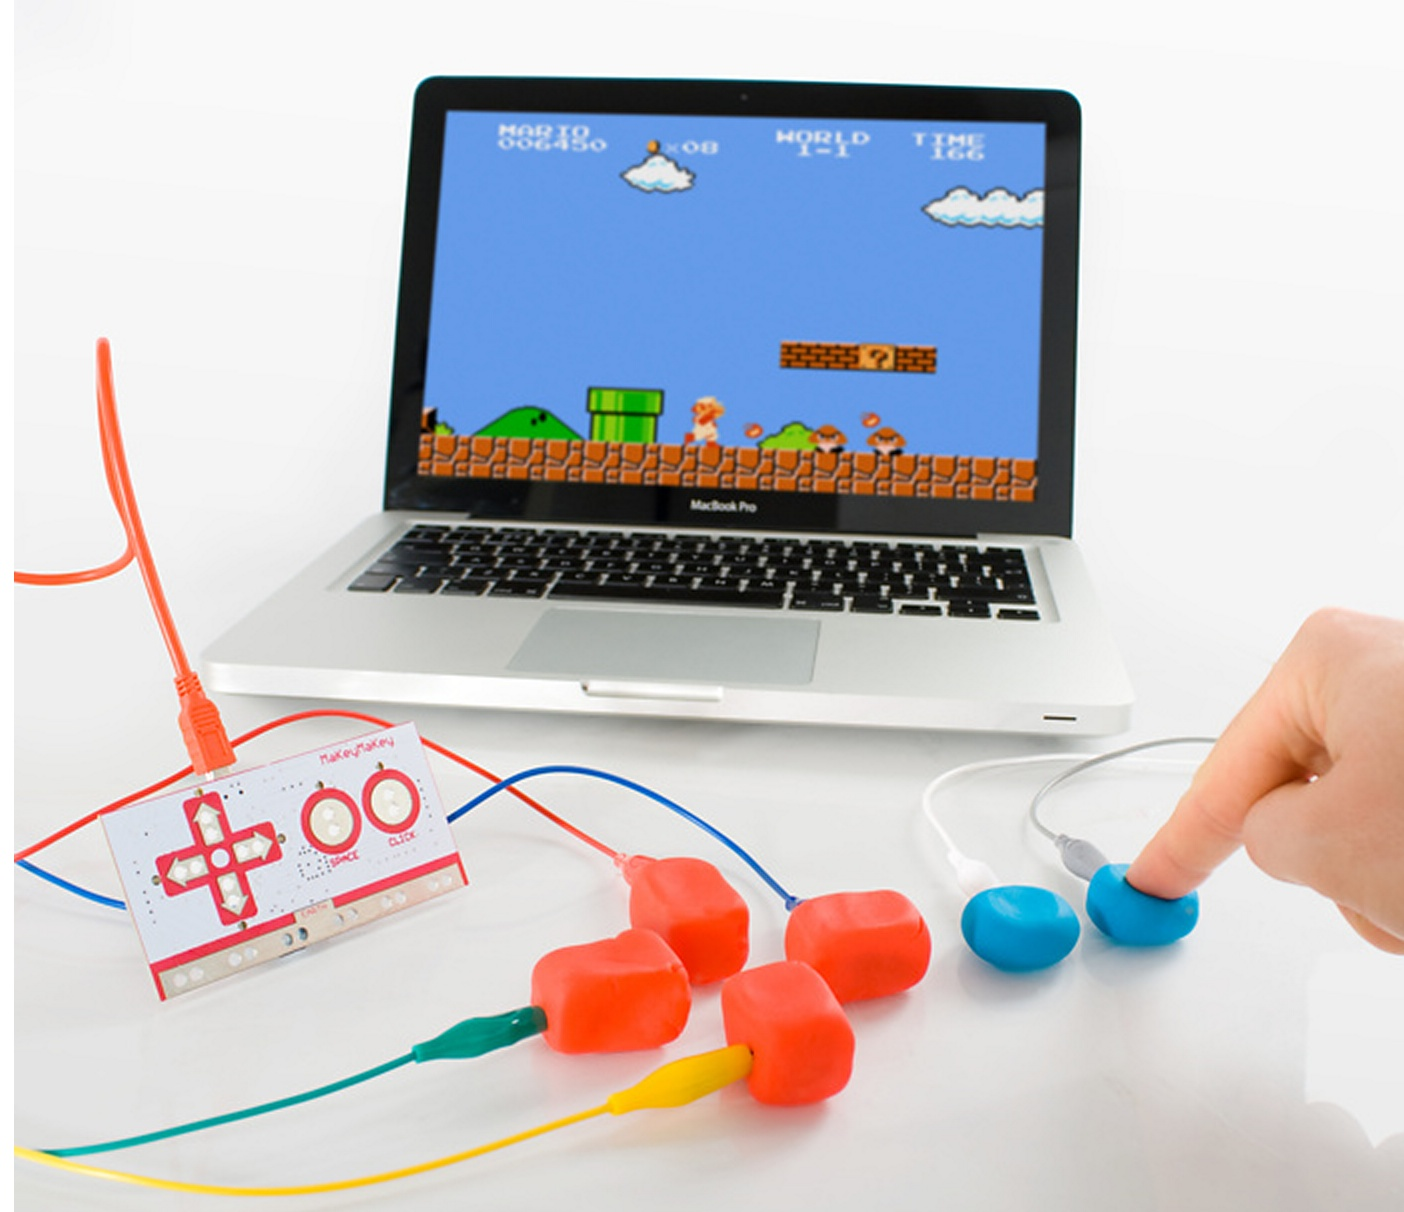
\includegraphics[height=24ex]{MakeyMakey.jpg}
\end{frame}

\begin{frame}{Heuristic Analysis Method}
	\begin{itemize}
		\item The cognitive approach is currently the dominant framework (or paradigm) for HCI (Perry, 2006).
		\item Players are characterised as `information processors', in which information undergoes a series of ordered processes
		in the player's mind.
		\item This worldview draws a comparison between the human brain and a computer; we can therefore model player activity in the same
		way that we model computer processing.
	\end{itemize}
\end{frame}

\begin{frame}{Heuristic Analysis Method}
	In a simple model of cognition, such as that proposed by Barber (1988), the process of cognition can be described as composing four sequential
	stages: 
	
	\vspace{2ex}

	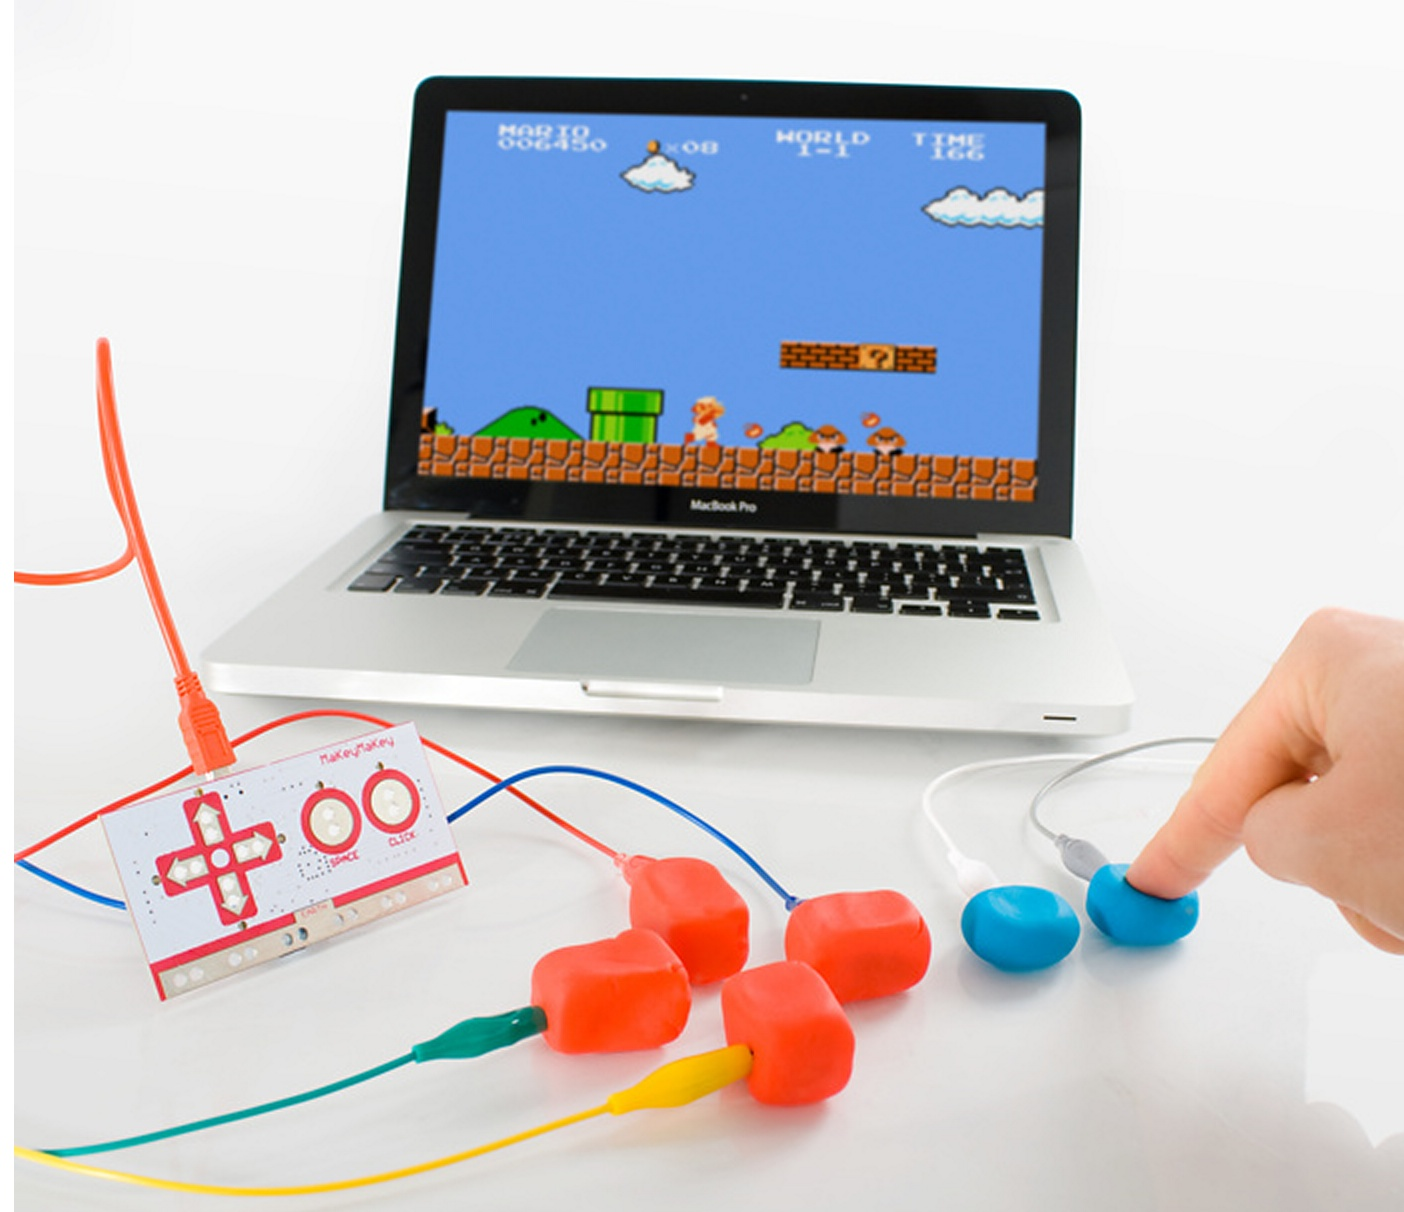
\includegraphics[height=24ex]{MakeyMakey.jpg}
\end{frame}